% *******************************************************************************
% * Copyright (c) 2007 by Elexis
% * All rights reserved. This document and the accompanying materials
% * are made available under the terms of the Eclipse Public License v1.0
% * which accompanies this distribution, and is available at
% * http://www.eclipse.org/legal/epl-v10.html
% *
% * Contributors:
% *    G. Weirich - initial implementation
% *
% *  $Id$
% *******************************************************************************
%
% !Mode:: "TeX:UTF-8" (encoding info for WinEdt)


\section{Grundkonfiguration}
Um das Programm nur mal auszuprobieren, brauchen Sie dieses Kapitel nicht durchzulesen. Der Standard-Installer von Elexis enthält eine eingerichtete Demo-Datenbank, die zum Testen ausreichend sein sollte.

Für die echte Programmanwendung kommen Sie allerdings um diese recht aufwändige Konfiguration nicht herum. Sie müssen 
dem Programm schliesslich alles mitteilen, was für Ihre Praxis spezifisch ist.

\subsection{Vorbemerkung}
Nehmen Sie sich bitte unbedingt genügend Zeit (mehrere Stunden bis einen ganzen Tag) für diese wichtigen Konfigurationsarbeiten. Wir 
empfehlen Ihnen, diese Anleitung auszudrucken und Schritt für Schritt durchzuführen.
Wenn Sie nicht sicher sind, wie die Konfiguration durchzuführen ist, empfehlen wir dringend, einen kompetenten Dienstleister damit zu beauftragen, da Fehler bei dieser Konfiguration die korrekte Arbeit später beeinträchtigen können. 

\subsection{Was Sie benötigen}
Bevor Sie mit der Konfiguration beginnen, sollten Sie die folgenden Daten zusammenstellen:
\begin{itemize}
  \item Namen, Benutzernamen und Passwörter für alle, die Elexis benutzen sollen
  \item Namen, ZSR-Nummern, EAN-Nummern, Bankverbindungen bzw. Postcheckkonto, ESR-Teilnehmernummern von allen Mandanten
  \item Eine Vorstellung, wie Ihr Briefkopf auf Briefen, Rezepten, AUF-Zeugnissen aussehen soll
  \item Eine Liste der in Ihrem Praxislabor durchgeführten Untersuchungen, eingeteilt in Gruppen
  \item Medikamentenliste ICD-10, Tarmed, Analysenliste, MiGel, soweit benötigt 
  \item EAN-Nummern der Krankenkassen und Unfallversicherer
\end{itemize} 
\subsection{Erster Schritt: Verbindung zur Datenbank herstellen}
Wenn Sie Elexis zum ersten Mal starten, wird eine lokale HSQL-Datenbank erstellt. In einer Einzelplatzumgebung können 
Sie damit bereits uneingeschränkt arbeiten. In einer Mehrbenutzerumgebung dagegen müssen Sie Elexis statt mit dieser 
lokalen Datenbank mit einer zentralen Server-Datenbank verbinden. Es wird im weiteren davon ausgegangen, dass der 
Server bereits installiert ist, läuft, und gemäss dem Vorschlag in
\href{http://www.elexis.ch/jp/index.php?option=content&task=view&id=72}{Datenbank} 
eingerichtet wurde. Starten Sie Elexis und wählen Sie im Hauptmenü
\textit{Datei-Verbindung}. 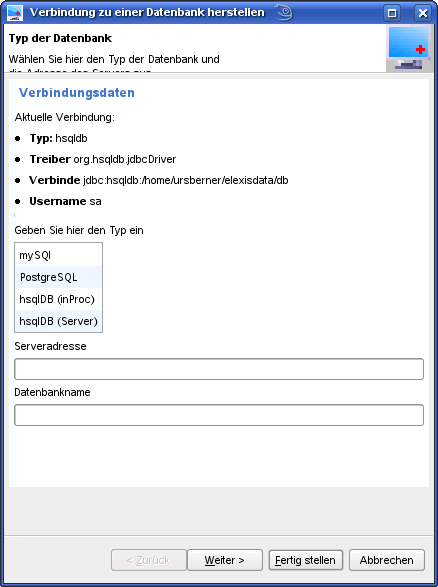
\includegraphics[width=3.5in]{images/verb1.png}
% verb1.png: 438x587 pixel, 72dpi, 15.45x20.71 cm, bb=0 0 438 587

Geben Sie Datenbanktyp, die TCP/IP-Adresse des Servers und den Namen der Datenbank ein und klicken Sie auf \textit{next}

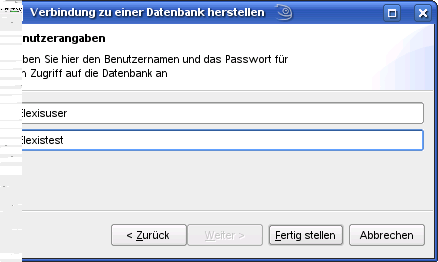
\includegraphics[width=3.5in]{images/verb2.png}
% verb2.png: 438x262 pixel, 72dpi, 15.45x9.24 cm, bb=0 0 438 262

Geben Sie schliesslich noch den Anwendernamen und das Passwort, so wie Sie es bei der Datenbankinstallation festgelegt haben ein, und klicken Sie auf \textit{finish}.
 Wenn alles korrekt ist, sollte jetzt Verbindung mit dem Server aufgenommen werden.

\subsection{\index{Mandant}Zweiter Schritt: Mandanten und Anwender einrichten}
Öffnen Sie die Perspektive \textit{Kontakte},

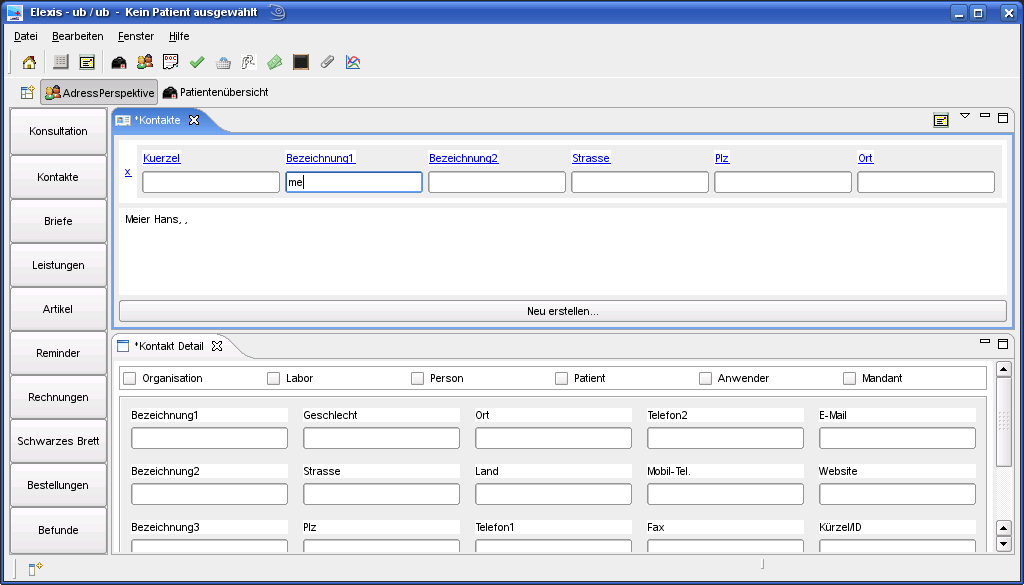
\includegraphics[width=4.5in]{images/grundkonfkonta.png}
% grundkonfkonta.png: 1024x585 pixel, 72dpi, 36.12x20.64 cm, bb=0 0 1024 585
\begin{itemize}
 \item Geben Sie unter \textit{Bezeichnung1} den Namen des neuen Mandanten oder Anwenders ein und klicken Sie auf
 \textit{Neu erstellen}
 \item Suchen Sie dann den eben erstellten Eintrag in der oberen Liste wieder auf, klicken Sie ihn an und ergänzen Sie 
 die Angaben in der unteren Hälfte. Wie immer bei Elexis brauchen Sie nicht unbedingt alle Felder auszufüllen. 
 \textit{Ernennen} Sie den eben erstellten Kontakt dann zum \textit{Mandanten} oder \textit{Anwender} (Ein Mandant ist 
 immer auch gleichzeitig ein Anwender, und beide sind immer auch \textit{Personen}
 \item Wenn Sie alle Mandanten und Anwender so eingegeben haben, gehen Sie auf Datei-Einstellungen und dort auf den 
 Reiter \textit{Zugriffsteuerung - Mandanten}
\end{itemize}

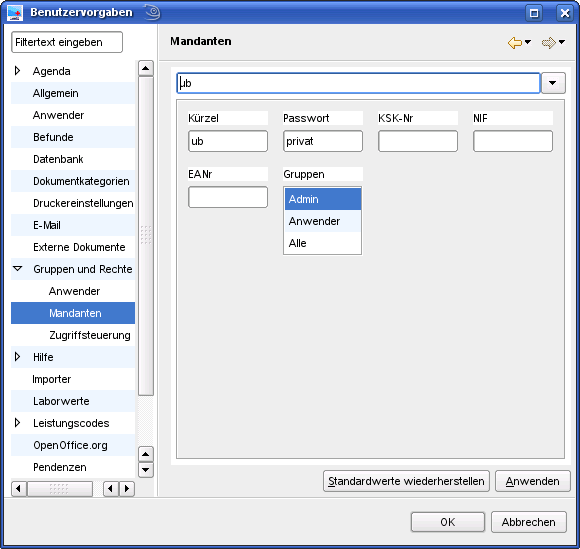
\includegraphics[width=4in]{images/grundkonfmand.png}
% grundkonfmand.png: 580x549 pixel, 72dpi, 20.46x19.37 cm, bb=0 0 580 549
\begin{itemize}
 \item Geben Sie dort die entsprechenden Angaben für Ihre eingerichteten Mandanten ein. Für \textit{Kürzel} muss der Anmeldename angegeben werden, für Passwort das Anmeldepasswort. Die restlichen Daten hängen vom Typ des Mandanten ab.
 \item Gehen Sie dann zum Abschnitt Zugriffsteuerung - Anwender
\end{itemize}

Geben sie dort für alle definierten \index{Anwender}Anwender die entsprechenden Daten ein. Vergessen Sie auch nicht, allen Anwendern einen existierenden Standard-Mandanten zuzuordnen (\textit{Für Mandant}). Auch für bereits angelegte Mandanten-Einträge (die Sie auch in der Anwender-Einstellung wiederfinden, da alle Mandanten auch Anwender sind), sollte ein Standard-Mandant festgelegt werden (Normalerweise er selbst). Der Zugeordnete Mandant definiert, in wessen Auftrag und auf wessen Rechnung der betreffende Anwender normalerweise arbeitet. Dies kann während der Arbeit geändert werden (Unter \textsc{Datei - Mandant}...), aber beim Einloggen wird immer zunächst der Standard-Mandant eingestellt.

\subsection{Dritter Schritt: Laborparameter eingeben}
Öffnen Sie zunächst wieder die \textit{Kontakte-View}. Geben Sie dort Ihr Eigenlabor und ihre externen Labors ein. 
Markieren Sie diese als \textit{Labor}

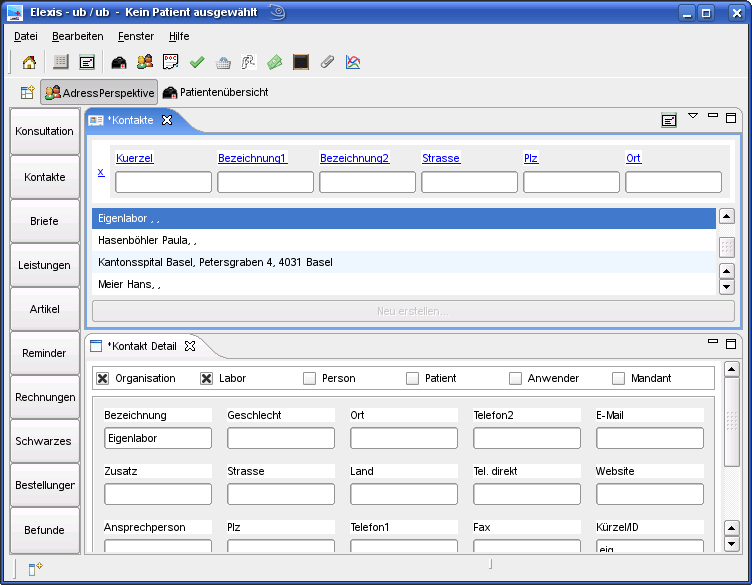
\includegraphics[width=4in]{images/grundkonfmand1.png}
% grundkonfmand1.png: 752x585 pixel, 72dpi, 26.53x20.64 cm, bb=0 0 752 585
\subsection{Vierter Schritt: Textprogramm konfigurieren}

Elexis arbeitet bisher nur mit OpenOffice zusammen. Deshalb wird hier auch nur die Konfiguration mit OpenOffice erläutert.
Wählen Sie in Elexis \textsc{Datei-Einstellungen-Textverarbeitung}

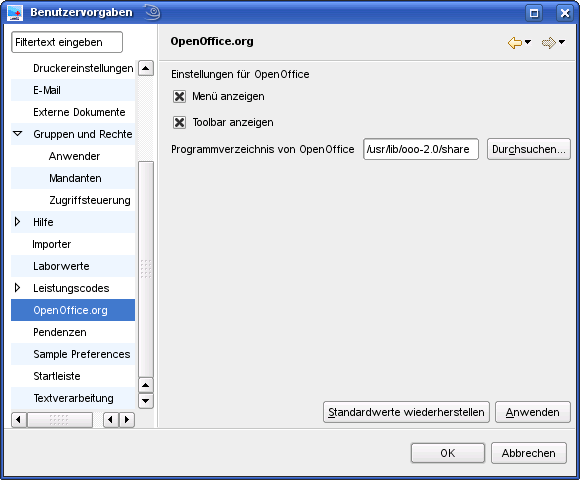
\includegraphics[width=3.5in]{images/grundkonfmand2.png}
% grundkonfmand2.png: 580x480 pixel, 72dpi, 20.46x16.93 cm, bb=0 0 580 480

\begin{itemize}
 \item Suchen Sie den Pfad des \textit{program} Unterverzeichnisses der OpenOffice Installation auf. Unter Windows wird das standardmässig in c:/programme/OpenOffice.org 2.0/program sein, bzw. an der Stelle, wo Sie OpenOffice installiert haben.
 \item Drücken Sie \textit{Apply}, Schliessen Sie die Konfiguration und starten Sie Elexis neu
 \item Wenn Sie jetzt z.B, die Briefe-Perspektive anwählen, sollte das Fenster von OpenOffice innerhalb des Elexis-Fensters erscheinen. (Dies wird beim ersten Mal recht lange dauern, d.h. ca. 30 Sekunden)
\end{itemize}

\subsubsection{Fünfter Schritt: \index{Vorlagen!Druckvorlagen}Druckvorlagen erstellen}
Für einige Formulare sucht Elexis nach vordefinierten Druckvorlagen mit einem festgelegten Namen. Diese definieren das für Ihre Anwendung spezifische Aussehen dieser Formulare. Es müssen jeweils Platzhalter für Variable Daten an den passenden Stellen eingefügt werden.

Um eine Formatvorlage zu erstellen, gehen Sie am besten so vor: Schreiben Sie die Vorlage ganz normal in der Textverarbeitung und speichern Sie sie als normales Textdokument. Von Elexis aus wählen Sie dann die Perspektive \textit{Briefe} und rufen das

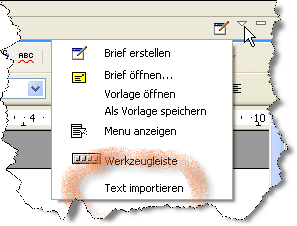
\includegraphics[width=2.5in]{images/import.png}
% import.png: 297x226 pixel, 96dpi, 7.86x5.98 cm, bb=0 0 223 169

ViewMenu rechts auf.

Wählen Sie dort \textit{Text importieren} und suchen Sie ihre vorher erstellte Vorlage auf.
 Hierdurch wird das Dokument nach Elexis importiert. Sie können jetzt noch Änderungen anbringen, rufen Sie dann wieder das ViewMenu rechts auf und wählen Sie diesmal \textit{Als Vorlage speichern}.

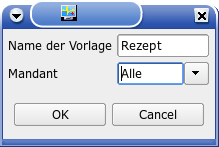
\includegraphics[width=2.5in]{images/rezept1.png}
% rezept1.png: 219x147 pixel, 72dpi, 7.73x5.19 cm, bb=0 0 219 147

Für \textit{Name der Vorlage} müssen Sie bei den unten aufgelisteten Standardvorlagen den entsprechenden Namen geben, für eigene Vorlagen können Sie beliebige Bezeichnungen einsetzen. Unter \textit{Mandant} können Sie einstellen, für welchen Mandanten diese Vorlage ist (oder ob für alle)

Im Folgenden jetzt eine Liste der erwarteten Standard-Vorlagen:

\begin{itemize}
\item Rezept: \index{Vorlagen!Rezept}Hierfür wird eine Formatvorlage mit dem Namen \textit{Rezept} benötigt. Diese kann z.B. so aussehen:
 \end{itemize}
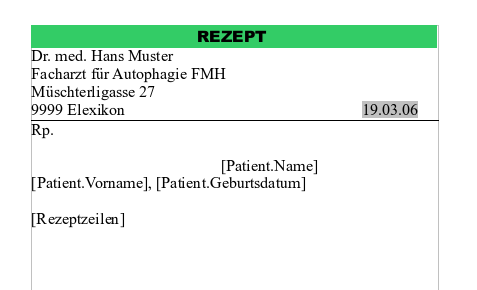
\includegraphics[width=4in]{images/rezept.png}
% rezept.png: 477x290 pixel, 72dpi, 16.83x10.23 cm, bb=0 0 477 290

An der Stelle, wo [Rezeptzeilen] steht, werden später die ausgewählten Medikamente eingesetzt. Dieser Platzhalter ist somit notwendig. Alle anderen Elemente der Vorlage \textit{Rezept} sind fakultativ.

\begin{itemize}
 \item \textit{AUF-Zeugnis}: Eine Formatvorlage für Arbeitszeugnisse. Als Platzhalter können [AUF.Grund], [AUF.von], [AUF.bis], [AUF.Prozent] und alle Standard-Platzhalter eingesetzt werden. Alle sind fakultativ.


 \item \textit{Laborblatt}: Für das Ausdrucken von Laborwerten. Die Laborwerte werden beim Platzhalter [Laborwerte] eingesetzt, dieser Platzhalter ist zwingend, andere können nach Wahl gesetzt werden.
\end{itemize}

\subsubsection{Sechster Schritt: Externe Datenbanken einlesen}

Eine Reihe von Stammdaten kann Elexis aus externen Quellen importieren. Beachten Sie bitte, dass diese Quellen mit 
einem Copyright versehen sein können, das Sie beachten müssen. Erkundigen Sie sich ggf. bitte bei der Stelle, die die 
Quellen veröffentlicht.

\begin{description}
 \item[Tarmed] \index{Stammdaten!Tarmed}Von \href{www.tarmedsuisse.ch}{Tarmed} kann eine Microsoft-Access-Datenbank 
 heruntergeladen werden. Binden Sie diese auf einem Windows-Computer als System-DSN ein. Gehen Sie in Elexis auf die 
 Perspektive  \textit{Codes} , wählen Sie dort den Reiter  \textit{Tarmed}  und rufen Sie das ViewMenu rechts auf. 
 wählen Sie den Eintrag  \textit{import}  und geben Sie die eben konfigurierte Tarmed-DSN ein. Je nach Geschwindigkeit 
 des PC wird der Import der gesamten Tarmed-Datenbank zwischen einer und 5 Minuten dauern. Eine detaillierte Anleitung 
 für den Import finden Sie hier
 \item[ICD-10] Von 
 \href{http://www.dimdi.de/dynamic/de/klassi/downloadcenter/icd-10-who/version2006/systematik/}{DIMDI} können Sie den 
 ICD-Katalog der WHO in computerlesbarer Form herunterladen. Sie benötigen die \textit{ICD-10-WHO-Systematik 
 EDV-Fassung ASCII} und die \textit{ICD-10-WHO-2006 Systematik Metadaten ASCII}. Entpacken Sie beide Zip's ins selbe 
 Verzeichnis. Die Warnung, dass eine Datei überschrieben wird, können Sie getrost ignorieren. Gehen Sie in Elexis auf 
 die \textit{Codes-Perspektive} und dort auf den Reiter  \textit{ICD-10}  und wählen Sie wieder  \textit{import}  aus 
 dem View-Menu. Geben Sie in der folgenden Dialogbox das Verzeichnis an, in das Sie den ICD-Code entpackt haben.
 \item[Medikamente und Medicals] \indexname{Stammdaten!Medikamente}Diese beiden Gruppen werden aus derselben Datenbasis 
 erstellt. Sie benötigen die Liste \textit{transfer.dat}, die Sie z.B. vom \textit{www.e-mediat.ch} im Abonnement 
 beziehen können. Wählen Sie die Perspektive  \textit{Codes} , dort den Reiter Medicals bzw. Medikamente, und dort 
 wieder im View-Menu die Option Import und geben Sie dort die den Pfad zur Transfer.dat-Datei an.
\textit{Anmerkung: Seit neuerem gibt es vom BAG eine Spezialitätenliste in Form einer Excel-Datei. Ein Importmodul für dieses Format ist in Vorbereitung; dann wird das kostenpflichtige transfer.dat nicht mehr benötigt  }
 \item[Analysenliste und MiGel] \index{Stammdaten!AL und MiGel}Diese werden vom BAG publiziert, allerdings leider aus 
 unverständlichen Gründen nur in PDF-Form. Es ist deshalb ein zusätzlicher und potentiell fehlerträchtiger 
 Konversionsschritt notwendig, um aus dieser PDF-Datei die Nutzdaten zu extrahieren. Sie benötigen dazu ein 
 entsprechendes Programm, unter Windows beispielsweise TextFromPDF, unter Linux z.B. xpdf. Erstellen Sie mit diesem 
 Hilfsprogramm eine plaintext-Version der Analysenliste, Gehen Sie in Elexis auf die Perspektive \textit{Codes}  und 
 dort auf den Reiter \textit{Analysen} bzw.MiGeL. Dort wieder den \textit{Import} aus dem ViewMenu aufrufen und den 
 Pfad der konvertierten Datei eingeben.
 \end{description}

\subsubsection{Siebter Schritt: Patientendaten einlesen bzw. eingeben}
Jetzt sind Sie mit den Vorbereitungen fertig und können mit dem Eingeben der eigentlichen Arbeitsdaten beginnen. Gehen 
Sie dazu für alle Patienten so vor, wie in der geführten Tour beschrieben

